\documentclass[main]{subfiles}

\begin{document}

\begin{definition}\label{Semigroup}
A \textbf{semigroup}\index{Semigroup} is a semicategory with a single object. A \textbf{monoid}\index{Monoid} $M$ is a category with a single object. A \textbf{group}\index{Group} is a monoid with all morphisms invertible. A \textbf{groupoid}\index{Groupoid} is a category with all morphisms invertible \par
A $G$ \textbf{set}\index{$G$ set} is a functor from $G$ to the category of sets. Equivalently, a \textbf{left group action}\index{Group action} is $G\times X\to X$, $(g,x)\mapsto g\cdot x$ satisfying $1\cdot x=x$, $g\cdot(h\cdot x)=(gh\cdot x)$, a right $G$ action is functor $G^{op}$ to the category of sets. A $G$ \textbf{space}\index{$G$ space} is a functor from $G$ to the category of topological spaces \par
An \textbf{equivariant map}\index{Equivariant map} of $G$ spaces is a natural transformation $f:X\to Y$
\begin{center}
\begin{tikzcd}
X \arrow[r, "f"] \arrow[d, "g"] & Y \arrow[d, "g"] \\
X \arrow[r, "f"]                & Y               
\end{tikzcd}
\end{center}
\end{definition}

\begin{definition}
The \textbf{center}\index{Center} of $G$ is $Z(G)=\left\{z\in G\middle|gz=zg,\forall g\in G\right\}$. $Z(G_1\times G_2)=Z(G_1)\times Z(G_2)$
\end{definition}

\begin{definition}
\textbf{Inner automorphism group}\index{Inner automorphism} of $G$ is $Inn(G)\leq Aut(G)$ consists of conjugations $x\mapsto gx g^{-1}$. \textbf{Outer automorphism group}\index{Outer automorphism} is $Out(G)=Aut(G)/Inn(G)$
\end{definition}

\begin{definition}
$G$ is \textbf{perfect}\index{Perfect group} if $[G,G]=G$
\end{definition}

\begin{definition}
A group action is \textbf{trivial}\index{Trivial action} if $g\cdot x=x$. A group action is \textbf{free}\index{Free action} if $g\cdot x=h\cdot x$ for some $x$ implies $g=h$, or equivalently. A group action is \textbf{transitive}\index{Transitive action} if $G\cdot x=X$. A free and transitive action is also called \textbf{regular}. A group action is \textbf{faithful}\index{Faithful action} if $\forall x\in X, G\cdot x\neq x$ \par
A \textbf{homogeneous space}\index{Homogeneous space} is a $G$ space with $G$ acting transitively
\end{definition}

\begin{definition}\label{Torsor}
A \textbf{torsor}\index{Torsor} $P$ is a set with an action $G\times P\to P, (g,p)\mapsto gp$ such that this action is free and transitive \par
When chosen an element $e\in P$, automatically you are giving it a group structure with $e$ as identity, notice $e: G\to P, g\mapsto ge$ is a bijection, suppose $g_pe=p$, then $g_e=1$, the group structure could be given as follows, $P\times P\to P, (p,q)\mapsto g_pg_qe$, and the inverse of $p$ is $g_p^{-1}e$. i.e. a torsor is a group forgetting its identity
\end{definition}

\begin{definition}
Let $X,Y$ be $G$ sets, the we can give $Y^X$ a $G$ set structure by $(gf)(x)=gf(g^{-1}x)$, it is easy to check that a map $f:X\to Y$ is equivariant iff $f$ is fixed under the $G$ action \par
Specially, if $G$ acts on $Y$ trivially, we have $(gf)(x)=f(g^{-1}x)$
\end{definition}

\begin{definition}
$H\leq G$ is a subgroup, $N\trianglelefteq G$ is a normal subgroup, $G=NH=N\rtimes H\text{ or }HN=H\ltimes N$ is the \textbf{semidirect product}\index{Semidirect product} and every $g\in G$ can be uniquely written as $nh$ or $hn$
\[(nh)(n'h')=n(hn'h^{-1})hh'\text{ or }(hn)(h'n')=hh'(h'^{-1}n'h')n'\]
\end{definition}

\begin{theorem}[Jordan-H\"older theorem]
Composition series is unique up to reordering
\end{theorem}

\begin{definition}
A \textbf{group representation}\index{Group representation} $V$ is a $\mathbb FG$ module
\end{definition}

\begin{definition}
Let $(\rho,V)$ be a group representation of finite group $G$, $W\leq V$ is called $G$ invariant if $GW\subseteq W$, namely, $W$ is $\mathbb FG$ submodule, then we get a subrepresentation on $(\rho|_W,W)$ of $G$, with $\rho|_W(g):=\rho(g)|_W$, if the only $G$ invariant subspace of $W$ are $0$ and $V$, we say $\rho$ is irreducible
\end{definition}

\begin{definition}
A group representation $(\rho,V)$ is completely reducible\index{Completely reducible representation}(semisimple) if $V=V_1\oplus\cdots\oplus V_n$, where $(\rho|_{V_i},V_i)$ are irreducible subrepresentations, namely, $V$ is the direct sum of simple $\mathbb FG$ modules
\end{definition}

\begin{definition}
Let $V$ be a complex vector space with Hermitian form $(,)$ finite group representation $(\rho,V)$ of $G$ is called unitary if $(\rho(g)v,\rho(g)w)=(v,w),\forall g\in G,v,w\in V$
\end{definition}

\begin{proposition}
Let $(\rho,V)$ be a unitary representation of $G$, $(\rho,V)$ is completely reducible
\end{proposition}

\begin{proof}
$W$ is $G$ invariant $\Rightarrow$ $W^\perp$ is $G$ invariant
\end{proof}

\begin{proposition}
Let $V$ be a complex vector space, $(\rho,V)$ is a representation, then there exists a positive definite Hermitian form on $V$ such that $(\rho,V)$ become a unitary representation
\end{proposition}

\begin{corollary}
Let $V$ be a complex vector space, a finite group representation $(\rho,V)$ is always completely reducible
\end{corollary}

\begin{definition}
Let $(\rho,V)$ be a representation of $G$, then the dual representation $(\rho^*,V^*)$ is defined as $\rho^*(g):=\rho(g^{-1})^{-T}$. The dual representation is chosen so that the following diagram commutes
\begin{center}
\begin{tikzcd}
V\otimes V^* \arrow[r, "\rho(g)\otimes\rho^*(g)"] \arrow[rd] & V\otimes V^* \arrow[d] \\
                                                             & k                     
\end{tikzcd}
\end{center}
\end{definition}

\begin{definition}
$H\subseteq G$, $(V,\pi)$ is a $H$ representation, the \textbf{induced representation}\index{Induced representation} is $\mathbb FG\otimes_{\mathbb FH}V$. Suppose $g_1,\cdots,g_n$ is a set of representatives of left cosets in $G/H$, $v_j$ is a basis for $V$, then $g_i\otimes v_j$ form a basis for $\mathbb FG\otimes_{\mathbb FH}V$. If $gg_i=g_jh$ for some $h\in H$, then $g(g_i\otimes v)=gg_i\otimes v=g_jh\otimes v=g_j\otimes hv$
\end{definition}

\begin{definition}
If $X$ is a right $G$ space, $Y$ is a left $G$ space, $X\times_GY$ is $X\times Y/\sim$, $(xg,y)\sim(x,gy)$. Equivalently, $X\times_G Y=X\times Y/G$ with left action $g(x,y)=(xg^{-1},gy)$ or right action $(x,y)g=(xg,g^{-1}y)$ \par
If $X,Y$ are left $G$ spaces, $X\times_G Y=X\times Y/G$ with left action $g(x,y)=(gx,gy)$ \par
If $X,Y$ are right $G$ spaces, $X\times_G Y=X\times Y/G$ with right action $(x,y)g=(xg,yg)$
\end{definition}

\begin{theorem}[Sylow's theorem]\index{Sylow's theorem}\label{Sylow's theorem}
$p$ is a prime, a $p$-group is a group consists of elements of order $p$-th power, a maximal one is a \textbf{Sylow} $p$\textbf{-subgroup} $P$ of $G$ which always exists by Zorn's Lemma \ref{Zorn's lemma}
\begin{enumerate}[label=\textbf{\arabic*.}, leftmargin=*]
\item If $|G|=p^nm$, $p\nmid m$, then $|P|=p^n$
\item Any subgroup of a Sylow $p$ subgroup is subconjugate to some other Sylow $p$ subgroup
\item $n_p=[G:N_G(P)]$, if the cojugacy class of $P$ is of order $n_p<\infty$, then $n_p\equiv 1\mod p$
\end{enumerate}
\end{theorem}

\begin{definition}
An \textit{isogeny}\index{Isogeny} is a morphism that is surjective with finite kernel
\end{definition}

\begin{definition}
A \textit{central extension}\index{Central extension} of $G$ is $1\to K\to C\to G\to1$, here $K\leq Z(C)$
\end{definition}

\begin{definition}
A \textit{stem extension}\index{Stem extension} of $G$ is $1\to K\to C\to G\to1$, here $K\leq Z(C)\cap C'$
\end{definition}

\begin{definition}
Denote $[n]=\{1,\cdots,n\}$, a \textbf{permutation}\index{Permutation} $[n]\xrightarrow\sigma[n]$ is a bijection, equivalently write $\sigma=\begin{pmatrix}
1&\cdots&n \\
\sigma(1)&\cdots&\sigma(n)
\end{pmatrix}$. $S_n=\mathrm{Aut}([n])$ is the permutation group \par
The \textbf{length} of $\sigma\in S_n$ is $|\sigma|$ is the number of $\sigma(i)<\sigma(j)$ while $i>j$
\end{definition}

\begin{definition}\label{Definition for shuffle}
Just like shuffling a deck of cards, $\sigma\in S_n$ is a $(p_1,\cdots,p_m)$\textbf{-shuffle}\index{Shuffle}, $p_1+\cdots+p_m=n$ if $\sigma(i)<\sigma(i+1)$ for $p_1+\cdots+p_k+1\leq i\leq p_1+\cdots+p_{k+1}$ \par
A $(p,q)$ shuffle can be represented by a path going only right or up from the lower left corner to the upper right corner in a $(p+1)\times(q+1)$ grid, $|\sigma|$ happen to be the number squares under the path
\end{definition}

\begin{example}[$(5,4)$ shuffles in $S_9$]
The red one is $\begin{pmatrix}
1&2&3&4&5&6&7&8&9 \\
2&5&7&8&9&1&3&4&6
\end{pmatrix}$. The blue one is $\begin{pmatrix}
1&2&3&4&5&6&7&8&9 \\
1&2&4&7&8&3&5&6&9
\end{pmatrix}$
\begin{center}
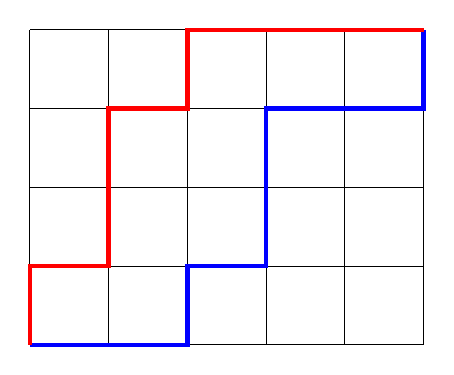
\begin{tikzpicture}
\foreach \x in {0,1,...,4}
{
\draw (0,\x)--(5,\x);
}
\foreach \x in {0,1,...,5}
{
\draw (\x,0)--(\x,4);
}
\draw[blue, ultra thick] (0,0)--(1,0)--(2,0)--(2,1)--(3,1)--(3,2)--(3,3)--(4,3)--(5,3)--(5,4);
\draw[red, ultra thick] (0,0)--(0,1)--(1,1)--(1,2)--(1,3)--(2,3)--(2,4)--(3,4)--(4,4)--(5,4);
\end{tikzpicture}
\end{center}
\end{example}

\begin{definition}
$G$ is a \textit{Coxeter group}\index{Coxeter group} if it has presentation
\[\left\langle r_1,\cdots,r_n\middle|(r_ir_j)^{m_{ij}}=1\right\rangle\]
$m_{ii}=1$(we should think of $r_i$'s as reflections), and $2\leq m_{ij}\leq\infty,\forall i\neq j$($m_{ij}=2$ means $r_i,r_j$ commutes). $S=\{r_1,\cdots,r_n\}$ is called a \textit{Coxeter system}\index{Coxeter system}, $G$ doesn't determine $S$. The \textit{Coxeter matrix}\index{Coxeter matrix} $M=(m_{ij})$ is symmetric, the corresponding \textit{Schl\"afli matrix} is $C_{ij}=-2\cos(\pi/m_{ij})$
\end{definition}

\begin{definition}
The \textit{Coxeter element}\index{Coxeter element} is the product of all simple reflections $s_i$'s, different order in multiplication give conjugation, the \textit{Coxeter number}\index{Coxeter number} is the order of the Coxeter element
\end{definition}

\begin{definition}
The \textit{Coxeter diagram}\index{Coxeter diagram} consists of $n$ nodes for $r_i$'s, there is an edge numbered $m_{ij}$ between $i$ and $j$ if $m_{ij}\geq3$(number $m_{ij}=3$ can just be omitted)
\end{definition}

\begin{theorem}
Finite Coxeter groups are classified by Coxeter diagram
\end{theorem}

\begin{proof}

\end{proof}

\begin{definition}[Grothendieck group]\label{Grothendieck group}
The \textbf{Grothendieck group}\index{Grothendieck group} of a commutative monoid $M$ is the abelian group $K$ and $i: M\to K$ satisfying universal property
\begin{center}
\begin{tikzcd}
M \arrow[rd, "f"] \arrow[d, "i", hook] &   \\
K \arrow[r, "\exists_1g"', dashed]               & A
\end{tikzcd}
\end{center}
For any abelian group $A$
\end{definition}

\begin{construction}
\[K=M\times M/\sim,\,M\xrightarrow i K, m\mapsto [m-0]\]
Abelian group $M\times M\cong\{[m-n]|m,n\in M\}$ is the set of formal differences with addition
\[[m_1-n_1]+[m_2-n_2]=[(m_1+m_2)-(n_1+n_2)]\]
$[0-0]$ is the identity and $[n-m]$ is the inverse to $[m-n]$
\[[m_1-n_1]\sim [m_2-n_2] \text{ if } m_1+n_2+m=m_2+n_1+m \text{ for some }m\in M\]
\end{construction}

\begin{construction}[Grothedieck completion]\index{Grothedieck completion}
\[K=F(M)/\sim,\,m+'n\sim(m+n)\]
$F(M)$ is the free abelian group generated by $M$ with addition $+'$
\end{construction}

\begin{definition}
The \textbf{Grothendieck group} of a semigroup $S$ is a group $K$ and $i: S\to K$ satisfying the universal property
\begin{center}
\begin{tikzcd}
S \arrow[rd, "f"] \arrow[d, "i", hook] &   \\
K \arrow[r, "\exists_1g"', dashed]               & G
\end{tikzcd}
\end{center}
Where $G$ is a group
\end{definition}

\begin{construction}
\[K=F(S)/\sim,\,m*'n\sim(m*n)\]
$F(S)$ is the free group generated by $S$ with multiplication $*'$
\end{construction}

\begin{definition}
$A$ is a unital $K$-algebra. The \textit{standard complex}\index{Standard complex} is
\[\cdots\to A\otimes A\otimes A\to A\otimes A\to A\to 0\]
with differentials
\[d_n(a_0\otimes\cdots\otimes a_{n+1})=\sum_{i=0}^n(-1)^ia_0\otimes\cdots\otimes a_ia_{i+1}\otimes\cdots\otimes a_{n+1}\]
Define $s_i:S^{i+2}(A)\to S^{i+3}(A)$, $a\mapsto1\otimes a$, $t_{i+1}:S^{i+3}(A)\to S^{i+2}(A)$, $\lambda\otimes a\mapsto\lambda a$, then $ts=1$, hence $s$ is a monomorphism. $d_n$'s are uniquely determined by $d_0(\lambda\otimes\mu)=\lambda\mu$, $ds+sd=1$, i.e. the identity map is null homotopic, hence the standard complex is a free $A$ bimodule resolution of $A$. If we denote $a_0\otimes\cdots\otimes a_{n+1}$ as $a_0[a_1|\cdots|a_n]a_{n+1}$, then
\[d_n[a_1|\cdots| a_{n}]=a_1[a_2|\cdots|a_n]+\sum_{i=1}^{n-1}(-1)^i[a_1|\cdots| a_ia_{i+1}|\cdots| a_{n}]+(-1)^n[a_1|\cdots|a_{n-1}]a_n\]
\end{definition}

\begin{example}
$d[a]=a[]-[]a$, $d[a|b]=a[]-[ab]+[]b$
\end{example}

\begin{definition}
The \textit{normalized standard complex}\index{Normalized standard complex} is with $A\otimes A/K\otimes\cdots\otimes A/K\otimes A$
\end{definition}

\begin{definition}
$R$ is a commutative ring, $C_*(G)$ is the tuple complex, equivalently, $B_*(G)$ is the bar resolution, $\bar B_*(G)=B_*(G)\otimes_{R[G]}R$. $B_*(G)$ is a differential graded algebra with shuffled product
\end{definition}

\begin{definition}
$R$ is a commutative ring, $M$ is right $R[G]$ module, $C_*(G)$ is the tuple complex, equivalently, $B_*(G)$ is the bar complex, $\bar B_*(G)=B_*(G)\otimes_{R[G]}R$, thus
\[M\otimes_{R[G]}B_*(G)\cong M\otimes_{R}R\otimes_{R[G]}B_*(G)\cong M\otimes_R\bar B_*(G)\]
Group homology with coefficients in $M$ is
\begin{align*}
H_k(G;M)&=H_k(M\otimes_{R[G]}C_*(G)) \\
&=H_k(M\otimes_{R[G]}B_*(G)) \\
&=H_k(M\otimes_{R}\bar B_*(G)) \\
&=\Tor_k^{R[G]}(M,R)
\end{align*}
The differential of $M\otimes_{R[G]} B_*(G)$ is given by
\begin{align*}
\partial(m\otimes[g_1|\cdots|g_n])&=\partial(m\otimes(1,g_1,g_1g_2,\cdots,g_1\cdots g_n)) \\
&=mg_1\otimes[g_2|\cdots|g_n]+\sum_{i=1}^{n-1}(-1)^im\otimes[g_1|\cdots|g_ig_{i+1}|\cdots|g_n] \\
&\mkern20mu+(-1)^nm\otimes[g_1|\cdots|g_{n-1}]
\end{align*}
$H_0(G;M)=M\otimes_{R[G]}R=M_G$. Write $H_k(G)$ for $H_k(G;\mathbb Z)$ \par
Group cohomology with coefficients in left $R[g]$ module $M$ is
\begin{align*}
H^k(G;M)&=H_k(\Hom_{R[G]}(B_*(G),M)) \\
&=\Ext^k_{R[G]}(R,M)
\end{align*}
The differential of $\Hom_{R[G]}(B_*(G),M)$ is given by
\begin{align*}
(d\phi)[g_1|\cdots|g_{n+1}]&=(d\phi)(1,g_1,g_1g_2,\cdots,g_1\cdots g_{n+1}) \\
&=\phi(\partial(1,g_1,g_1g_2,\cdots,g_1\cdots g_{n+1})) \\
&=g_1\phi[g_2|\cdots|g_{n+1}]+\sum_{i=1}^{n}(-1)^i\phi[g_1|\cdots|g_ig_{i+1}|\cdots|g_{n+1}] \\
&\mkern20mu+(-1)^{n+1}\phi[g_1|\cdots|g_n]
\end{align*}
$H^0(G;M)=\Hom_{R[G]}(R,M)=M^G$. Write $H^k(G)$ for $H^k(G;\mathbb Z)$ \par
\end{definition}

\begin{remark}
A right $R[G]$ module $M$ can be viewed as a left $R[G]$ module and vice versa via $g^{-1}m=mg$
\end{remark}

\begin{definition}
The \textit{augmentation ideal}\index{Augmentation ideal} is the kernel of the augmentation map $R[G]\to R$
\end{definition}

\begin{definition}
A \textit{derivation} or \textit{crossed homomorphism}\index{Crossed homomorphism} is $D:G\to M$ such that $D(gh)=gD(h)+D(g)$, this can be identified with $Z^1(G;M)$. $D_m(g)=gm-m$ are \textit{principal derivations}, this can be identified with $B^1(G;M)$
\end{definition}

\end{document}